\documentclass[xcolor=dvipsnames,aspectratio=169]{beamer}

% INCLUSIÓN DOS PAQUETES IMPRESCINDIBLES DE IDIOMA E CODIFICACIÓN DE CARACTERE.
\usepackage[T1]{fontenc}
\usepackage[english]{babel}
\usepackage[utf8]{inputenc}
\usepackage{csquotes}

%ACRONYMS para engadir un glosario de acronimos automatizado
% \usepackage[acronyms,nonumberlist,nopostdot,nomain,nogroupskip]{glossaries}
% \input{./acronyms.tex}

% PAQUETES PARA FIGURAS E GRAFICOS
\usepackage{graphicx}
%   \usepackage[pdftex]{graphicx}
  \usepackage{epstopdf}
   \graphicspath{{./img/}}
  % and their extensions so you won't have to specify these with
  % every instance of \includegraphics
   \DeclareGraphicsExtensions{.eps,.pdf,.png,.jpg}   
\usepackage{subfigure}
\usepackage{caption}
\usepackage[inkscapelatex=false]{svg}

%Tikz plots
\usepackage{tikz}
\usepackage{tikzscale}
\usepackage{tikz-network}
\usetikzlibrary{plotmarks,patterns,decorations.pathreplacing,backgrounds,calc,arrows,arrows.meta,spy,matrix,backgrounds,shapes}

\tikzset{
    block/.style = {draw, rectangle, 
        minimum height=1cm, 
        minimum width=1.2cm},
    input/.style = {coordinate,node distance=1cm},
    output/.style = {coordinate,node distance=2cm},
    arrow/.style={draw, -latex,node distance=1.5cm},
    pinstyle/.style = {pin edge={latex-, black,node distance=1.5cm}},
    sum/.style = {draw, circle, node distance=1cm}
}
\newcommand{\tikzmark}[1]{\tikz[overlay,remember picture] \UE (#1) {};}
\newcommand{\DrawBox}[4][]{%
    \tikz[overlay,remember picture]{%
        \coordinate (TopLeft)     at ($(#2)+(-0.4em,1.6em)$);
        \coordinate (BottomRight) at ($(#3)+(0.4em,-1.0em)$);
        %
        \path (TopLeft); \pgfgetlastxy{\XCoord}{\IgnoreCoord};
        \path (BottomRight); \pgfgetlastxy{\IgnoreCoord}{\YCoord};
        \coordinate (LabelPoint) at ($(\XCoord,\YCoord)!0.5!(BottomRight)$);
        %
        \draw [red,#1] (TopLeft) rectangle (BottomRight);
        \UE [below, #1, fill=none, fill opacity=1] at (LabelPoint) {#4};
    }
}
\newcommand*\circled[1]{\tikz[baseline=(char.base)]{
            \node[shape=circle,draw,inner sep=1.3pt] (char) {#1};}}
\usepackage{pgfplots}
\pgfplotsset{compat=newest}
\pgfplotsset{plot coordinates/math parser=false}
\usepgfplotslibrary{patchplots,groupplots}

% OUTROS PAQUETES DE USO COMUN. HOXE EN DIA OS COMPILADORES SON TAN RAPIDOS QUE EU METO TODOS SEMPRE
% \usepackage{float}
% \usepackage{ucs} 
% \usepackage{subcaption}
\usepackage{psfrag}
\usepackage{verbatim}
\usepackage{amsmath}
\usepackage{amsfonts} 
\usepackage{amssymb} 
\usepackage{amsthm}
\usepackage{pifont}
\usepackage{array}
\usepackage{listings}
\usepackage{stfloats}
\usepackage{algorithm} 
\usepackage{algorithmic} 
\usepackage{url} 
\usepackage{enumerate}
\usepackage{multirow}
\usepackage{wasysym}
\usepackage{cancel}
\usepackage{lmodern}
\usepackage{mathrsfs}

\input{EETbeamerconfig.tex}
\input{mydefinitions.tex}

%---------------
% LIMIAR
%---------------
%configuracion de opcions de beamer persoais, pero alleas ao estilo

% COMANDO QUE INTRODUCE UNHA DIAPOSITIVA CUN ÍNDICE NO QUE APARECEN VELADAS TÓDALAS SECCIÓNS MENOS A ACTUAL. ÚTIL PARA INTRODUCIR OS TÍPICOS ÍNDICES INTERMEDIOS.
\newcommand{\Inter}{\frame{\tableofcontents[currentsection]}}
\newcommand{\inter}{\frame{\tableofcontents[currentsection,currentsubsection]}}

% Pes de imaxe
\renewcommand{\figurename}{Fig.}
\addto\captionsenglish{\renewcommand{\figurename}{Fig.}}
\setbeamertemplate{caption}[numbered]

%ESTE PAQUETE PERMITE POÑER A BIBLIOGRAFIA AO PE DE PAXINA CON CONFIGURACIONS ESTETICAS PERSOAIS
% \usepackage[style=ieee,doi=false,isbn=false,url=true,backend=bibtex]{biblatex}
% \bibliography{./bibliografia.bib}
% \newrobustcmd*{\footfullcitenomark}{%
%   \AtNextCite{%
%     \let\thefootnote\relax 
%     \let\mkbibfootnote\mkbibfootnotetext
%     }%
%   \footfullcite}

%paquete para engadir notas de guion ao pdf
\usepackage{pgfpages}
% \setbeameroption{show only notes} 
% \setbeameroption{show notes}
% \setbeameroption{show notes on second screen=right}
% DATOS DO DOCUMENTO
\title{Advanced Communication Systems}
\subtitle{Part 2.5:\\ Multi-user Communications:\\ Spectrum and Co-existence}
\author[FGC]{Felipe G\'omez Cuba}
\institute[XX]{
\begin{columns}[T]
\begin{column}{9cm}\centering
Despacho 204\\
Titorías: Lun-Xov 15:00-16:30\\
(En caso de confinamento: videochamada a calquera horario acordado)\\
  \texttt{gomezcuba@gts.uvigo.es}\\
\end{column}
\end{columns}
}

\date{19 \& 24 November 2020 }

\begin{document}

% Diapositiva co título
%\frame[plain]{\titlepage}%the ``classic'' beamer cover pageç

\frame{\frametitle{\\}%generate top bar, but blank line as tittle
\titlepage
}%approximation to the ``GPSC ppt'' cover page, but with central beamer title

% \frame{\tableofcontents}
% \note[itemize]{%itemized notes are special ``note'' slides that beamer can append to the pdf or not, depending on a boolean toggle option
% \item Introduce yourself
% \item In this work we studied blablabla.
% }

% \section{IAB MmWave Network}

\frame[allowframebreaks]{\frametitle{Spectrum Coexistence Introduction}
 Spectrum is a \textbf{very scarce commonality}
\begin{figure}
 \centering
 \includegraphics[width=.6\columnwidth]{USA_allocation}
%  \caption{USA spectrum allocation}
\end{figure}
\begin{itemize}
 \item Separation of licensed in different bands
 \item Interference limited networks: $\uparrow$ bandwidth $\Rightarrow$ $\uparrow$ capacity
\end{itemize}
\pagebreak

 \textcolor{ARust}{YET MOST LICENSED BANDS ARE EMPTY MOST OF THE TIME}
\begin{figure}
 \centering
 \includegraphics[width=.55\columnwidth]{whitespaces}
 \caption{Spectrum use in rural/airport/metropolitan areas (Ofcom)}
\end{figure}
\begin{itemize}
 \item Emergency services, government, scientific
 \item Services with variable demand in time or location
\end{itemize}
}

\frame{\frametitle{Cognitive Radio Definition}
 \begin{definition}[Cognitive Radio]
  A radio that knows the environment and self-adapts to it
 \end{definition}
 In industry, 99$\%$ of the time it is assumed to mean
    \begin{definition}[Dynamic Spectrum Access]
    \begin{itemize}
    \item An incumbent (licensed) \textbf{primary user} does not use its spectrum all the time or in all locations.
    \item A cognitive (unlicensed) \textbf{secondary user} enters the licensed band opportunistically
    \end{itemize}
    \end{definition} 
        \begin{figure}         
              \begin{tikzpicture}[scale=.7, transform shape]
                \node[draw,circle] (x1) at (0,1.5) {PT};
                \node[draw,circle] (x2) at (0,0) {ST};
                \node[draw,circle] (y1) at (5,1.5) {PR};
                \node[draw,circle] (y2) at (5,0) {SR};
                \draw [->,ARust] (x1) -- (y1);
                \draw [->,dotted,gray] (x1) -- node[anchor=north,pos=0.65] {$\beta_P$} (y2);
                \draw [->,dashed,KYJade] (x2) -- node[anchor=south,pos=0.65] {$\beta_S$} (y1);
                \draw [->,dashed,VCobalt] (x2) -- (y2);
            \end{tikzpicture}
        \end{figure}      
}


\frame{\frametitle{Underlay Cognitive Radio}
\begin{itemize}
 \item Cognition: noise and interference at PR\\ \ \\
 \item Interference Channel: \textit{Very weak interference regime}\\ \ \\
 \item Example: Ultra WideBand (UWB) technologies\\ \ \\
 \item Problem: \textbf{collective total interference}
\end{itemize}

\begin{figure}
            \begin{tikzpicture}[scale=1]
                \draw [->] (0,0) -- node [anchor=east] {$P$} (0,2.1);
                \draw [->] (0,0) -- node [anchor=north] {$t$} (8,0);                
                \draw[pattern=dots,opacity=.50] (0,0) rectangle  (8,.5);
                \node[anchor=east] at (0,.25) {Max Intf.};            
                \draw[ARust,fill,fill opacity=.25] (1,0) rectangle node {PT} (3,2);     
                \draw[ARust,fill,fill opacity=.25] (4.25,0) rectangle  node {PT} (6.5,1.75);       
                \draw[VCobalt,fill=VCobalt,fill opacity=.25] (.5,0) rectangle node {ST} (2,.4);  
                \draw[VCobalt,fill=VCobalt,fill opacity=.25] (2.5,0) rectangle node {ST} (5,.4);  
                \draw[VCobalt,fill=VCobalt,fill opacity=.25] (6,0) rectangle (7.5,.4);   
            \end{tikzpicture}         
    \caption{Underlay Cognitive Radio}
    \end{figure}



}

\frame{\frametitle{Overlay Cognitive Radio}
\begin{itemize}
 \item Cognition: \textbf{primary transmitted message and interf.}
 \item \textit{Relay Channel}: \textcolor{KYJade}{reinforce} the primary signal
 \item \textit{Gel'fand-Pinsker Channel}: Dirty Paper Coding
 \item Many technical difficulties
 \item Example: Possible in DVB-T, but difficult
\end{itemize}

\begin{figure}
            \begin{tikzpicture}[scale=1]
                \draw [->] (0,0) -- node [anchor=east] {$P$} (0,2.5);
                \draw [->] (0,0) -- node [anchor=north] {$t$} (8,0);                
                \draw[pattern=grid,opacity=.50] (0,0) rectangle (8,.5);
                \node[anchor=east] at (0,.25) {Old Max Intf.};          
                \draw[pattern=dots,opacity=.5] (0,0) rectangle (8,.9);
                \node[anchor=east,KYJade] at (0,.75) {New Max Intf.};        
                \draw[ARust,fill,fill opacity=.25] (1,0) rectangle (3,2);     
                \draw[ARust,fill,fill opacity=.25] (4.25,0) rectangle (6.5,1.75);       
                \draw[KYJade,fill,fill opacity=.25] (1,2) rectangle (3,2.4);     
                \draw[KYJade,fill,fill opacity=.25] (4.25,1.75) rectangle (6.5,2.15);       
                \draw[VCobalt,fill=VCobalt,fill opacity=.25] (.5,0) rectangle (2,.8);  
                \draw[VCobalt,fill=VCobalt,fill opacity=.25] (2.5,0) rectangle (5,.8);  
                \draw[VCobalt,fill=VCobalt,fill opacity=.25] (6,0) rectangle (7.5,.8);   
            \end{tikzpicture}      
    \caption{Cooperative Relaying Overlay}          
    \end{figure}
}

\frame[allowframebreaks]{\frametitle{White Spaces (Interweave) Cognitive Radio}

\begin{itemize}
 \item Cognition: \textbf{white spaces} (original CR inspiration)
 \item Problem: identify gaps in time, frequency and space (MIMO)
 \item \textit{Binary Hypothesis Testing:} detect if primary is present
 \item \textit{Spectrum Database:} simply ask the authority
 \item IEEE 802.22 Wireless Regional Area Network (WRAN) standard
\end{itemize}

% \begin{figure}
%             \begin{tikzpicture}[scale=1]
%                 \draw [->] (0,0) -- node [anchor=east] {$P$} (0,2.5);
%                 \draw [->] (0,0) -- node [anchor=north] {$t$} (8,0);                
%                 \draw[pattern=dots,opacity=.50] (0,0) rectangle (8,.5);
%                 \node[anchor=east] at (0,.25) {Max Intf.};          
%                 \draw[ARust,fill,fill opacity=.25] (1,0) rectangle (3,2);     
%                 \draw[ARust,fill,fill opacity=.25] (4.25,0) rectangle (6.5,1.75);       
%                 \draw[VCobalt,fill=VCobalt,fill opacity=.25] (0.1,0) rectangle (0.9,1.3);  
%                 \draw[VCobalt,fill=VCobalt,fill opacity=.25] (3.1,0) rectangle (4.15,1.3);  
%                 \draw[VCobalt,fill=VCobalt,fill opacity=.25] (6.6,0) rectangle (7.5,1.3);   
%             \end{tikzpicture}            
%     \end{figure}
\begin{figure}
    \begin{tikzpicture}[scale=.8]
        \draw [->] (0,0) -- node [anchor=east] {$P$} (0,3,0);
        \draw [->] (0,0) -- node [anchor=north] {$t$} (10,0,0);
        \draw [->] (0,0) -- node [anchor=south east] {$f$} (0,0,-5);
        \def\drawmybox[#1](#2,#3,#4)(#5,#6,#7)%
        {% [draw options] (x,y,z) (sizex,sizey,sizez)
            \draw[#1] (#2,#3,#4-#7) -- ++(#5,0,0) -- ++(0,#6,0) -- ++(-#5,0,0) -- cycle;
            \draw[#1] (#2,#3,#4) -- ++(0,0,-#7) -- ++(0,+#6,0) -- ++(0,0,#7) -- cycle;
            \draw[#1] (#2,#3,#4) -- ++(#5,0,0) -- ++(0,#6,0) -- ++(-#5,0,0) -- cycle;
            \draw[#1] (#2+#5,#3,#4) -- ++(0,0,-#7) -- ++(0,+#6,0) -- ++(0,0,#7) -- cycle;
            \draw[#1] (#2,#3+#6,#4) -- ++(+#5,0,0) -- ++(0,0,-#7) -- ++(-#5,0,0) -- cycle;
        }
        \drawmybox[pattern=dots](0,0,0)(10,.25,5)
        
        \drawmybox[TAMustard,fill,fill opacity=.25](.8,0,-2.6)(4,.8,2)
        \drawmybox[VCobalt,fill,fill opacity=.25](4.9,0,-2.6)(1.4,.6,2)
        \drawmybox[TAMustard,fill,fill opacity=.25](6.5,0,-2.6)(1.5,1.1,2)
        \drawmybox[VCobalt,fill,fill opacity=.25](8.1,0,-2.6)(1.5,.6,2)
        
        \drawmybox[VCobalt,fill,fill opacity=.25](.1,0,-.1)(.8,.6,2)
        \drawmybox[ARust,fill,fill opacity=.25](1,0,-.1)(2,1,2)
        \drawmybox[VCobalt,fill,fill opacity=.25](3.1,0,-.1)(1.05,.6,2)
        \drawmybox[ARust,fill,fill opacity=.25](4.25,0,-.1)(2.25,.875,2)
        \drawmybox[VCobalt,fill,fill opacity=.25](6.6,0,-.1)(2,.6,2)
    \end{tikzpicture}            
    \caption{Dynamic Spectrum Access}
    \end{figure}    
}

\frame{\frametitle{Hybrid Approaches: Cooperative Spectrum Leasing}
\begin{itemize}
 \item Cognition: \textbf{primary transmitted message and \textit{spectral efficiency}}
 \item Create white spaces via cooperation
 \item Problem: Requires VBR primary with a MAC protocol
\end{itemize}

\begin{figure}
 \subfigure[Before]{
    \includesvg[width=.35\textwidth]{CSLprinciples_before}
    }
 \subfigure[With CSL]{
    \includesvg[width=.35\textwidth]{CSLprinciples_after}
    }
\end{figure}
}


\frame{\frametitle{Network Slicing}
\begin{columns}
 \begin{column}{6cm}
  \begin{itemize}
   \item Operator spectrum resale\\ \ \\
   \item Centralized: no uncertainty\\ \ \\
   \item Each Slice may specify
   \begin{itemize}
    \item Virtual Private Network core
    \item OFDMA radio resources
    \item Service Level Agreement
    \item Mobile Edge Computing\\ \ \\
  \end{itemize}
   \item Problem: oligopoly, neutrality
  \end{itemize}
 \end{column}
 \begin{column}{7cm}
  \begin{figure}
    \centering
    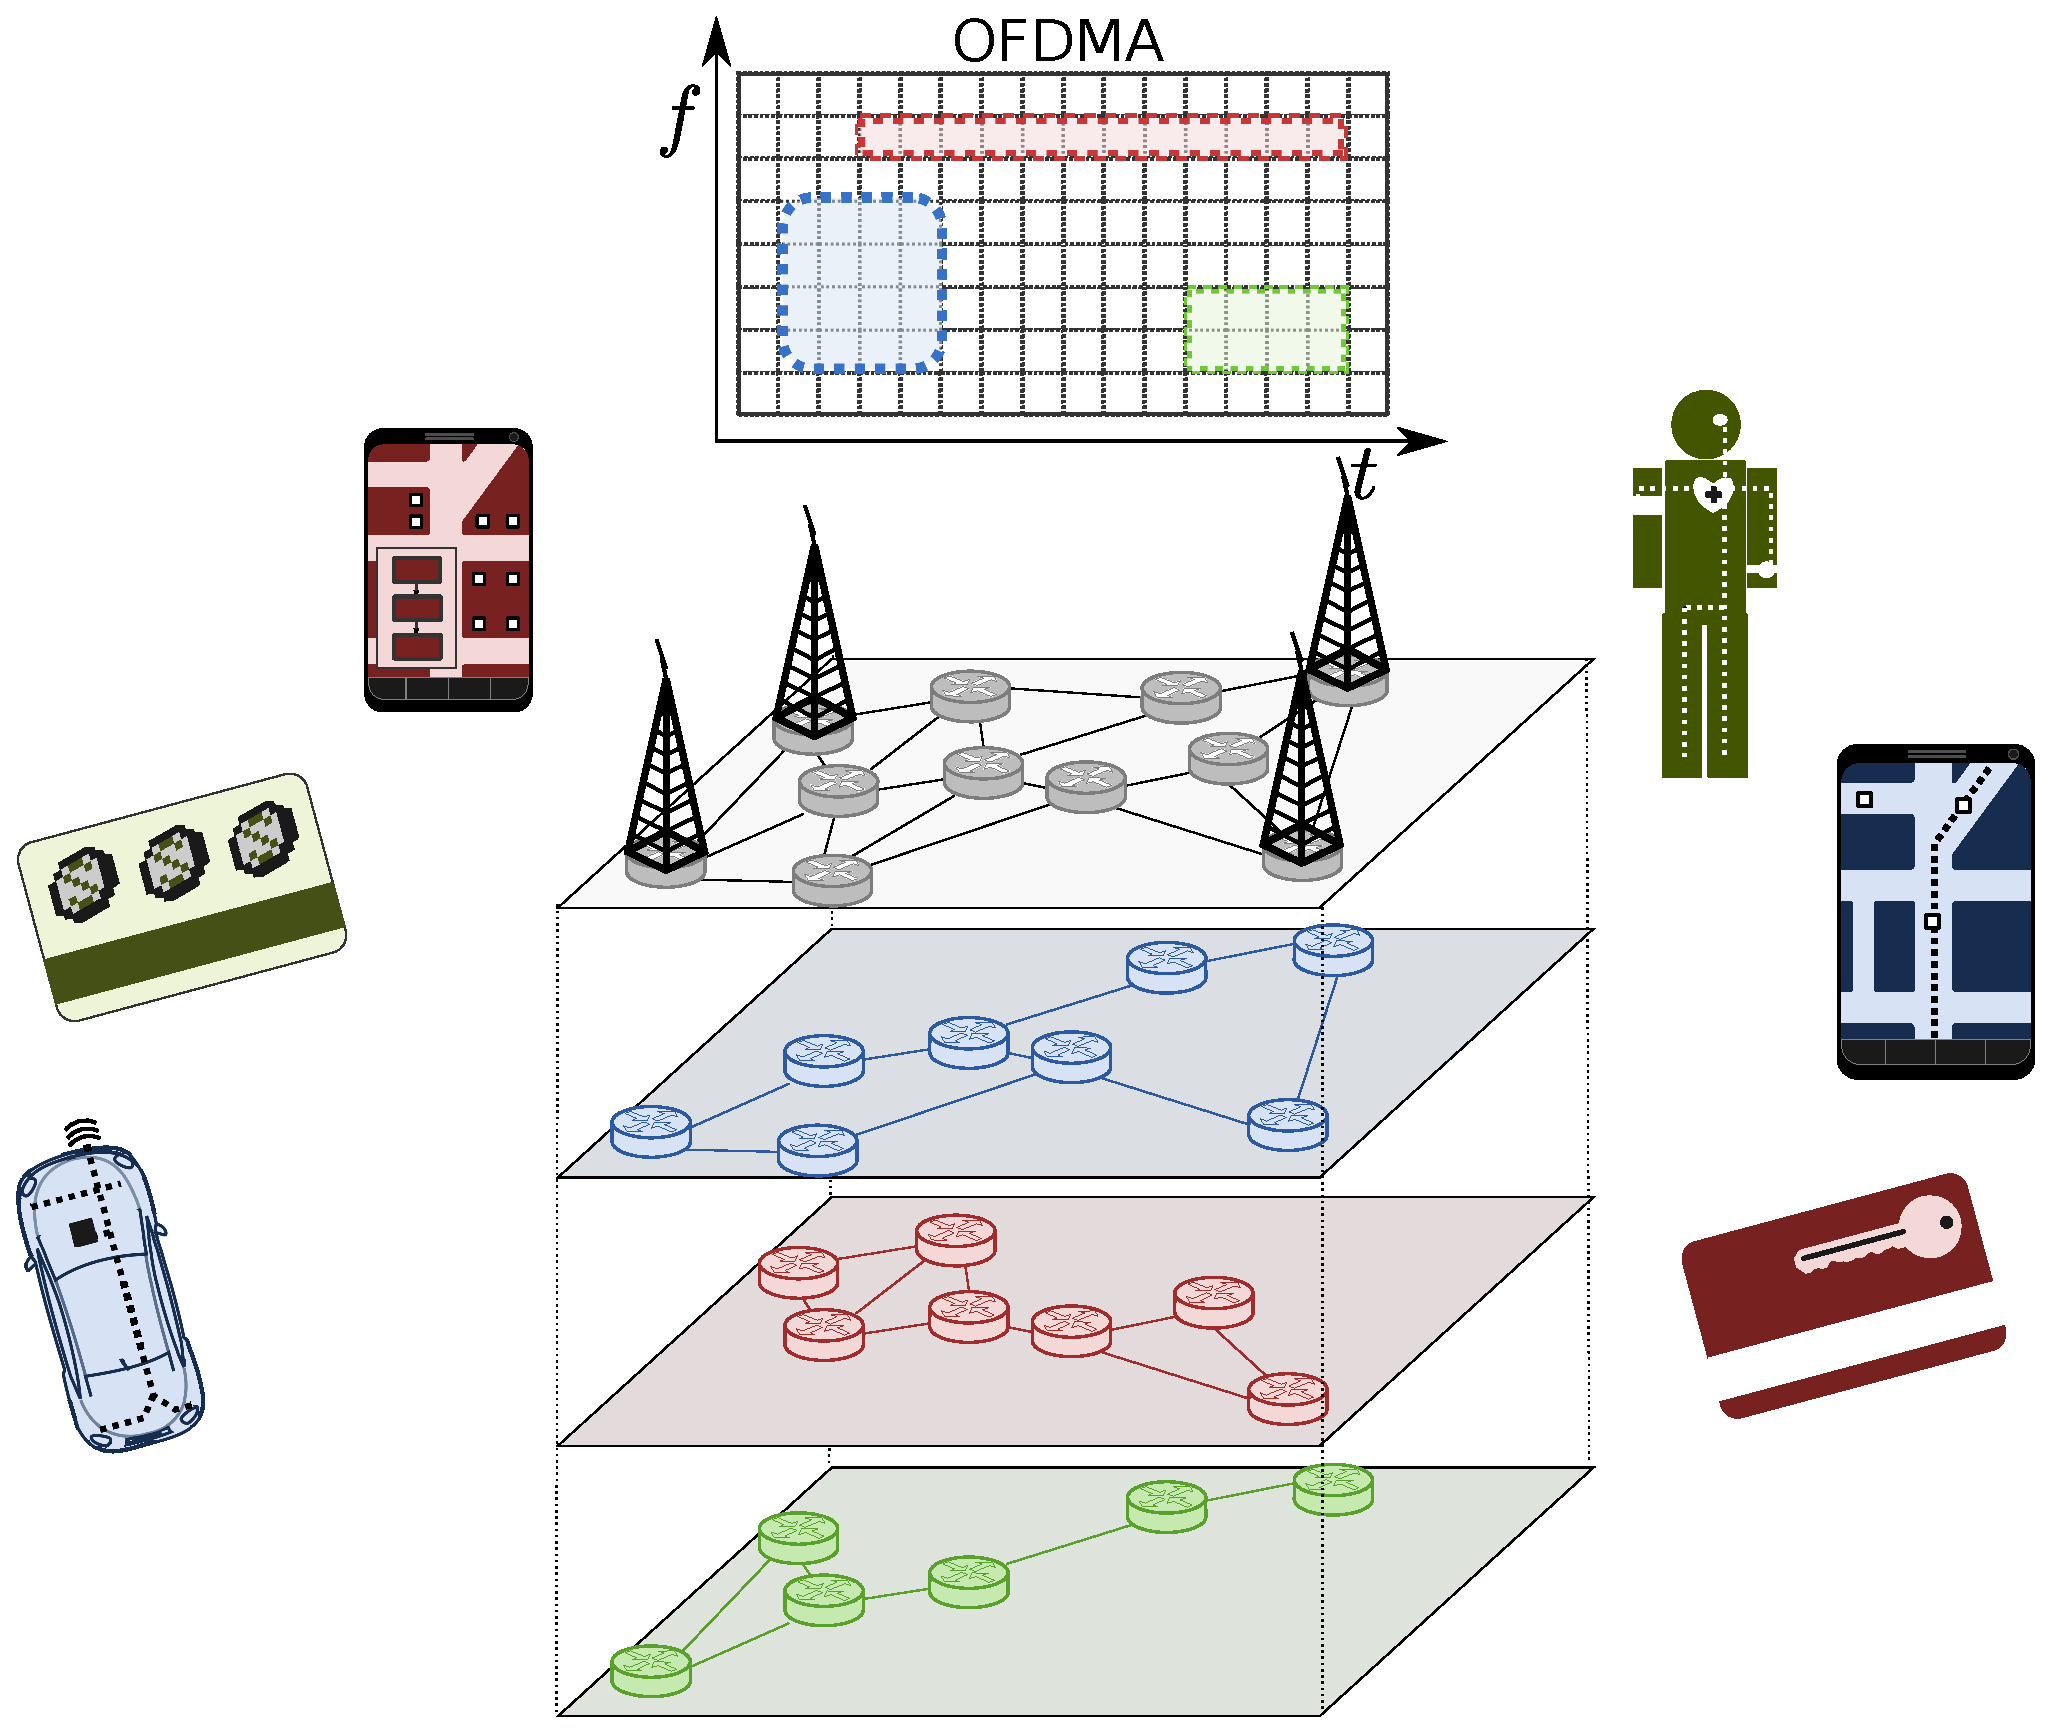
\includegraphics[width=\columnwidth]{networkslicing}
    \caption{Network with 3 slices}
\end{figure} 
 \end{column}
\end{columns}
}

\frame[allowframebreaks]{\frametitle{Spectrum Sensing Motivation}

\begin{tabular}{r|lll}
                & Database          & N. Slicing       & Cognitive Radio  \\ \hline
Criterion       & \textcolor{KYJade}{\Large \cmark} Query \& register & \textcolor{ARust}{\Large \xmark} Pay2play     & \textcolor{ARust}{\Large \xmark} Interference \\
Hardware        & \textcolor{KYJade}{\Large \cmark} Low complexity    & \textcolor{gray}{\Large ?} Centralized   & \textcolor{gray}{\Large ?} Distributed   \\
Agility         & \textcolor{ARust}{\Large \xmark}  Slow               & \textcolor{KYJade}{\Large \cmark} Market        & \textcolor{KYJade}{\Large \cmark} Local Area\\
Fairness        & \textcolor{KYJade}{\Large \cmark} Public Regulator    & \textcolor{ARust}{\Large \xmark} Oligopoly      & \textcolor{KYJade}{\Large \cmark} Contention/Coop. \\ \hline
Sensing    & \textcolor{KYJade}{\Large \cmark} Law enforcement  & \textcolor{KYJade}{\Large \cmark}Enhancement & \textcolor{ARust}{\Large \xmark} Indispensable \\
\end{tabular}

\pagebreak

\begin{itemize}
\begin{columns}
 \begin{column}{6cm}
 \item \textbf{Underlay}
    \begin{itemize}
        \item Primary or Secondary
        \item Detect excess interference at PR
        \item $1$ ST exceeds power regulation
        \item $N$ STs too many, even if compliant\\ \ \\
    \end{itemize}    
 \item \textbf{Interweave}: 
    \begin{itemize}
        \item Secondary only
        \item Find White Space 
        \item Monitor sideband ($\simeq$ Underlay)
        \item Detect primary return
    \end{itemize}  
 \end{column}
 \begin{column}{6cm}  
 \item \textbf{Overlay}+DPC: 
    \begin{itemize}
        \item Primary or Secondary
        \item Find PT with CSI(S)T (how?)
        \item PT unaware
        \item Mon. interference ($\simeq$Underlay)\\ \ \\
    \end{itemize}
 \item \textbf{Overlay}+Relaying: 
    \begin{itemize}
        \item Secondary only
        \item Find PT with low SE
        \item PR \textbf{aware} $\succ$ unaware
        \item Reward division (Game Theory)
    \end{itemize}  
 \end{column}
\end{columns}
\end{itemize}  
}

\frame[allowframebreaks]{\frametitle{Interference Temperature}
    \begin{itemize}
     \item SINR $\gamma_k = \frac{P_{1ry}}{\sum_{i=1}^{N_I}P_{i}+BN_o}$ for large $N_I$
    \begin{itemize}
        \item ZF/IC is impractical
        \item $\sum_{i=1}^{N_I}P_{i} \approx \mathcal{CN}$ by CLT\\ \ \\
    \end{itemize}    
    \item Thermal noise: $N_o=k T$
    \begin{itemize}
        \item $k=$ Boltzmann constant $=1.38064852 \times 10^{-23}$ (J/K)
        \item $T=$ temperature (K)
        \item Standard atmospheric $-174$ dBm/Hz @ $23^o$C\\ \ \\
    \end{itemize}
    \begin{definition}[Interference Temperature]
     A simplified measure of the total interference assuming CLT and TIN
         $$T_I=\frac{\sum_{i=1}^{N_I}P_{i}}{k W}$$
    \end{definition}
    
    \pagebreak
    \item
    \begin{algorithmic}
     \IF{$T_I<$ threshold $T_L$}
        \STATE {Primary and secondary transmissions can coexist in that band}
     \ELSE
        \STATE {Secondary must stop interfereing (How?)}
     \ENDIF
    \end{algorithmic}
    \item Problem: suppose we receive
    $$y(t) = x(t)+x_i(t)+z(t),$$
    with unknown $x(t)$ and $x_i(t)$. How do we determine if a received Watt of $y(t)$ belongs to $x(t)$ or to $x_i(t)$?
    \begin{itemize}
        \item Known primary $x(t)$ statistics
        \item Measuring $T_I$ during primary silence
    \end{itemize}
    \end{itemize}
}   


\frame{\frametitle{Sensing Spectrum Properties}
\begin{itemize}
\begin{columns}[T]
 \begin{column}{6cm}
    \item Energy sensing
        \begin{itemize}        
         \item Energy threshold $\eta$ improves the more we know about $x(t)$
         $$E_y=\Ex{}{y(t)}$$
         \item \texttt{If $E_y>\eta$ then primary=True}\\ \ \\
        \end{itemize}
    \item Coherent sensing
        \begin{itemize}
         \item $x(t)$ known $\forall t\in[0,T]$
         $$C_y(t)=\int_{0}^{T}x^*(\tau)y(t+\tau)d\tau$$
         \item \texttt{If $C_y(t)>\eta\to$ True}
        \end{itemize}
 \end{column}
 \begin{column}{6.5cm}
  \item Cyclostationarity sensing
    \begin{itemize}
        \item All artificial signals cyclostationary
        \begin{align*}\textnormal{Example: }\Ex{}{x(t)}&=\Ex{}{x(t+T)}\\
         &\neq\Ex{}{x(t+0.47T)}
        \end{align*}
        \item \texttt{If isWSS($y$) then primary=False}\\ \ \\
     \end{itemize}
    \item Autocorrelation detection
    \begin{itemize}
        \item Assume $x(t)$ is WSS      
        $$R_y(\Delta t)=\Ex{}{y^*(t)y(\Delta t+t)}$$ 
        \item \texttt{If $R_y(\Delta t)>\eta\to$ True}
    \end{itemize}
 \end{column}
\end{columns}
\end{itemize}
}

\frame[allowframebreaks]{\frametitle{Detection theory}
\begin{definition}[Binary Hypothesis Testing]
Field of statistics that studies estimation of a single event or binary choice
\begin{enumerate}
\item $H_0$: There is no event (no primary signal, we are only measuring noise) 
\item $H_1$: There is an event (primary signal plus noise) 
\end{enumerate}
\end{definition}
\begin{itemize}
 \item Denote $\hat H$ the decided hypothesis\\ \ \\
 \item Errors of type...
    \begin{enumerate}[I]
    \item {\bf False Positives aka False Alarms:} $\hat H = H_1$ when $H_0$ is true ($P_{FA}$)
    \item {\bf False Negative aka Missed Detection:} $\hat H=H_0$ when $H_1$ is true ($P_{MD}$)
    \end{enumerate}
 \item Frequently used alternative notation $P_D=1-P_{MD}$
\pagebreak
\item Performance of any detector as a 2D chart $(P_{FA},P_{D})$
\item Random guess $\frac{1}{2}\to$ worst case performance
\end{itemize}

\begin{columns}[T]
 \begin{column}{4cm}
  \textbf{Example:}
  \begin{itemize}
   \item $H_0$: $y\sim \mathcal{N}(0,\sigma^2)$
   \item $H_1$: $y\sim \mathcal{N}(\mu,\sigma^2)$\\ \ \\
   \item $\hat{H}=H_1$ \texttt{if} $y>Y_T$\\ \ \\
   \item $P_{FA}=\mathscr{Q}(Y_T)$
   \item $P_{D}=1-\mathscr{Q}(\mu-Y_T)$\\ \ \\
   \item $P_{MD}=\mathscr{Q}(\mu-Y_T)$
   \item $P_{TN}=1-\mathscr{Q}(Y_T)$
  \end{itemize}

 \end{column}
 \begin{column}{8cm}
  \begin{figure}
  \centering
    \colorbox{white}{\includegraphics[width=.9\textwidth]{ROC.png}}
    \caption{Receiver Operating Characteristic}
  \end{figure}
 \end{column}
 \end{columns}
}

\frame[allowframebreaks]{
\frametitle{BHT Detection as an Optimization}
\begin{itemize}
\item Multi-objective optimization
\item Low $P_{FA}$ and large $P_D$\\ \ \\
\item Marginal method:  {\bf Neyman-Pearson criterion} 
\begin{itemize}
\item Maximize $P_D$ with maximum accepted $P_{FA}$
$$  \max P_D \textnormal{ s.t. }  P_{FA} \leq \alpha $$
\item Equivalent to Log-likelihood threshold
    $$\Lambda \doteq \log \frac{f_y(y|H_1)}{f_y(y|H_0)} $$
\item $\hat{H}=H_1$ \textit{if} $\Lambda \geq \eta$ and $H_0$ otherwise\\ \ \\
\item $\eta$ chosen to guarantee constraint $P_{FA}<\alpha$ (Lagrange multiplier)\\ \ \\
\end{itemize}
\pagebreak
\item Linear combination method:  \textbf{Bayes risk minimization}
\begin{itemize}
\item Assign costs $C_{ij}$ to the different errors
\begin{equation*}
\min R \triangleq C_{00} p_0 P_{TN}+C_{10}p_0 P_{FA} + C_{01} p_1 P_{MD} + C_{11} p_1 P_D
\end{equation*}
\item with a-priori probabilities $p_1=P(H_1)$, $p_0=P(H_0)$\\ \ \\
\item and complementaries $P_D=1-P_{MD}$, $P_{TN}=1-P_{FA}$\\ \ \\
\end{itemize} 
\item In the cognitive radio, $P_{MD}$ and $P_{FA}$ are not equally important. Why? 
\end{itemize} 
}

\frame[allowframebreaks]{\frametitle{Energy Sensing Performance}
\begin{itemize}
\item One of the simplest detectors
\item Assume $N$ (possibly complex) captured samples $y_0, \cdots, y_{N-1}$
\begin{equation*}
E_y\triangleq \Ex{}{|y(t)|^2}\simeq \frac{1}{N} \sum_{n=0}^{N-1} |y_n|^2\to \hat{H}=H_1 \texttt{if} E_y \geq \eta
\end{equation*}
\item If $H_0$ is true, $\Ex{}{E_y}=\sigma_z^2$ (zero-mean noise is assumed)
\item If $H_1$ is true, $\Ex{}{E_y}=E\{|x(t)|^2\} + \sigma_z^2=P_{1ry} +  \sigma_z^2$ (assuming noise and signal uncorrelated)\\ \ \\
\item Fails when model parameters $P_{1ry}$ and $\sigma_z$ unknown
\begin{itemize}
\item Unknown good threshold value
\item Solved by looking at signal features (out of the scope of this course)\\ \ \\
\end{itemize}
\item To compute $P_{FA}$ and $P_{MD}$ we need the statistical distributions
\begin{itemize}
\item $f(E_y|H_0)$ is a sum of $2N$ squares of i.i.d. Gaussians (i.e., $\mathcal{N}(0, \sigma_z^2/2N)$) (complex-valued signals), i.e. a Chi-square distribution
    $$ P_{FA} =\int_{\eta}^{\infty} f(E_y|H_0) d E_y \textnormal{ where } E_y|H_0 \sim \chi_{2N}^{2}(\frac{\sigma_z^2}{2N})$$
\item We can assume $x(t)\approx$ Gaussian, and therefore $f(E_y|H_1)$ is another Chi-square
$$P_{MD} =\int_0^{\eta} f(E_y|H_1) d E_y \textnormal{ where } E_y|H_1 \sim \chi_{2N}^{2}(\frac{P_{1ry}+\sigma_z^2}{2N})$$
\item These integrals can be solved semi-analytically\\ \ \\
\end{itemize}
\item Alternatively, for large $N$ we can use CLT to approximate $\chi^2$s as Gaussian
\begin{eqnarray*}
\frac{2}{\sigma_z^2} \sum_{n=0}^{N-1} |w_n|^2 &\sim& {\mathcal N}(2N, 4N) \\
\frac{2}{\sigma_z^2+P} \sum_{n=0}^{N-1} |y_n|^2 &\sim& {\mathcal N}(2N, 4N)
\end{eqnarray*}
\begin{eqnarray*}
P_{FA} &\approx & Q \left( \sqrt{N} \frac{\eta- \sigma_z^2}{\sigma_z^2} \right) \\
P_{MD} &\approx& 1- Q \left( \sqrt{N} \frac{\eta - (\sigma_z^2+P)}{\sigma_z^2+P} \right)
\end{eqnarray*}
\end{itemize}
}


\frame{\frametitle{Homework: Energy Sensing}

Plot the 2D performance curve of $P_FA$ vs $P_{MD}$ of a basic energy detector for a channel 
$$y=x+z$$
where the signal is 
$$x\begin{cases}\sim \mathcal{CN}(0,\sigma_z^2)&\textnormal{ with probability }0.5\\
    0 \textnormal{ otherwise}
   \end{cases}$$
and the noise is $z\sim\mathcal{CN}(0,\sigma_z^2)$ with $\sigma_z^2=10^{-2}$.

Implement a simple energy threshold $\eta$ with $N=1$ samples, plot the performance line by Monte-Carlo simulation in the 2D plane as you vary the threshold value, repeat the plot for $N=100$, and compare the results with the approximate $Q()$ function analytical values. 
}

\frame{\frametitle{The Problem of Unknown Noise}
\begin{itemize}
\item Primary SNR $\gamma_{1ry} \doteq P_{1ry}/\sigma_z^2$
\item Minimum num. samples to achieve $P_{FA}, P_{MD}$
\begin{equation*}
N  = [Q^{-1}(P_{FA}) - Q^{-1} (1-P_{MD}) (1+\gamma)^2] \gamma^{-2}
\end{equation*}
\item Unknown $\sigma_z^2\in [(1/\varepsilon)\hat{\sigma}_w^2, \varepsilon \hat{\sigma}_w^2]$
\begin{eqnarray*}
P_{FA}^{max} &\approx & Q \left( \sqrt{N} \frac{\eta- \varepsilon \sigma_z^2}{\varepsilon \sigma_z^2} \right) \\
P_{MD}^{max} &\approx& 1- Q \left( \sqrt{N} \frac{\eta - (\varepsilon^{-1} \sigma_z^2+P)}{\varepsilon^{-1} \sigma_z^2+P} \right)
\end{eqnarray*}
\item low-SNR approximation 
\begin{equation*}
N  \stackrel{\gamma \to 0}{=} [Q^{-1}(P_{FA}^{max}) - Q^{-1} (1-P_{MD}^{max})] \cdot [\gamma-(\varepsilon-\varepsilon^{-1})]^{-2}
\end{equation*}
\item \textcolor{ARust}{$P_{1ry} \leq (\varepsilon-\varepsilon^{-1}) \sigma_z^2\to$ no finite-$N$ detector exists}
\end{itemize}
}

\frame{
\frametitle{Cooperative sensing}

\textbf{Cognitive Radio $\to$ anyone may transmit}\\ \ \\
\begin{columns}[T]
 \begin{column}{6cm}
  Conventional contention MAC
    \begin{itemize}
        \item Multiple simultaneous STs\\ \ \\
        \item Compete with each other\\ \ \\
        \item $\neq$ hardware capabilities\\ \ \\
        \item $\neq$ interests and goals
    \end{itemize}
 \end{column}
 \begin{column}{6cm}
  Cooperative Cognitive Networks
    \begin{enumerate}
    \item Coordinated network access
    \begin{itemize}
     \item Optimize Throughput,
     \item Reduce Interference, etc.\\ \ \\
    \end{itemize}
    \item Distributed spectrum sensing
    \begin{itemize}
     \item \textcolor{KYJade}{\Large \cmark} Improved performance
     \item \textcolor{KYJade}{\Large \cmark} Overcome fading
     \item \textcolor{KYJade}{\Large \cmark} No \textbf{hidden nodes}
     \item \textcolor{ARust}{\Large \xmark} tx. situational info.
     \item \textcolor{ARust}{\Large \xmark} data fusion complexity
    \end{itemize}
    \end{enumerate}   
 \end{column}
\end{columns}
}
 
\frame{\frametitle{Fading and Hidden Node}
\begin{columns}
 \begin{column}{6cm}
  \begin{figure}
   \centering
   \colorbox{white}{\includegraphics[trim={6cm 0 0 0},clip,width=\textwidth]{Distributed_sensing.jpg}}
   \caption{Fading}
  \end{figure}
 \end{column}
 \begin{column}{6cm}
  \begin{figure}
   \centering
   \colorbox{white}{\includegraphics[trim={.25cm .25cm 1.5cm .25cm},clip,width=\textwidth]{hiddennode.png}}
   \caption{Hidden Node}
  \end{figure}
 \end{column}
\end{columns}
}

\frame{
\frametitle{Possible topologies}

\begin{enumerate}[a]
\begin{columns}[T]
 \begin{column}{6cm}
    \item \textbf{Centralized system}
\begin{itemize} 
 \item Central processor (fusion center)
 \item Rec. info. from all sensors
 \item Makes estimations \& decisions
\end{itemize}
 \end{column}
 \begin{column}{6cm}
  \item \textbf{Decentralized system}
\begin{itemize} 
 \item Nodes are intelligent
 \item Data fusion and processing
\end{itemize}
\item \textbf{Decentralized multi-hop}
\begin{itemize}
 \item $\uparrow$ Decision delays
\end{itemize}
 \end{column}
\end{columns}
\end{enumerate}
  \begin{figure}
   \centering
   \colorbox{white}{\includegraphics[width=0.7\textwidth]{topologies.jpg}}
  \end{figure}
}

\frame{
\frametitle{How to fuse the information?}
\begin{itemize}
\begin{columns}[T]
 \begin{column}{6cm}
 \item Sensor information
 \begin{itemize}
  \item Hard (boolean)
  \item Soft (energy, LLRs)
  \item Compressed (\texttt{summary(}soft\texttt{)})\\ \ \\
 \end{itemize}
 \end{column}
 \begin{column}{6cm}  
 \item Usually assumed indep. observ.
 \begin{itemize}
  \item in time
  \item in space
 \end{itemize} 
 \end{column}
\end{columns}
\begin{columns}[T]
 \begin{column}{13cm}
\item $N_s$ sensors with boolean decision $u_i$ \textcolor{ARust}{with known $(P_{FA,i},P_{MD,i})$}
\begin{equation*}
\log \Lambda(\uu) = \sum_{i=1}^{N_s} u_i \log \frac{1-P_{MD,i}}{P_{FA,i}}+ (1-u_i) \log \frac{1-P_{FA,i}}{P_{MD,i}}
\end{equation*}
 \end{column}
\end{columns}
\begin{columns}[T]
 \begin{column}{6cm}
\item Computationally simple
\begin{itemize}
    \item Boolean logic (OR, AND...)
    \item Voting (Majority, K-out-of-N...)
\end{itemize}
 \end{column}
 \begin{column}{6cm}   
\item Soft information improvements
\begin{itemize}
 \item Estim. statistics (mean, var.,etc.)
 \item Neyman-Pearson's $\to$ sum LLRs
 \end{itemize}
 \end{column}
\end{columns}
\end{itemize}
} 

\frame{
\frametitle{Cooperative energy fusion}
\begin{itemize}
\item $i$-th sensor energy estim. $E_i = \sum_{n=0}^{N-1} |y_{i,n}|^2$ with $y_{i,n} = h_i x_n + z_{n,i}$\\ \ \\
\begin{columns}[T]
 \begin{column}{4cm}
    \item Linear fusion center
    \begin{equation*}
    E_f=\sum_{i=1}^{N_s} a_i E_i
    \end{equation*}
 \end{column}
 \begin{column}{8cm}
    \begin{itemize}
        \item Optimal Likelihood: $a_k^*=|h_i|^2/(|h_i|^2+1)$
        \item Equal Gain Combining: $a_i$ identical
        \item Maximal Ratio Combining: $a_i=|h_i|^2$
        \item Marginal opt.: $\min_{a_i} P_{MD} \textnormal{ s.t. } P_{FA}\leq \alpha$\\ \ \\
    \end{itemize}
 \end{column}
\end{columns}
    \item Non-linear fusion methods, p.e. 
        $$E_f=\max_i S_i$$
    \item Threshold @ fusion energy
     $$\hat{H}=H_1 \texttt{ if } E_f>\eta$$
\end{itemize}
}

\frame{\frametitle{Sequential detection}
\begin{itemize}
\item Long {\em Sensing time} $\to$ missed brief spectrum opportunities\\ \ \\
\item Minimize the detection time s.t. $P_{FA},P_{MD}$ constraints\\ \ \\
\begin{columns}[T]
 \begin{column}{6cm}
    \item Wald sequential test
    \begin{itemize}
    \item $\Lambda_n$ Likelihood up to $n$
    \item 2 thresholds $\eta_1=\frac{1-\beta}{\alpha}\; \eta_0=\frac{1-\alpha}{\beta}$
    \item $P_{FA}\leq \frac{\alpha}{1-\beta}$, $P_{MD} \leq \frac{\beta}{1-\alpha}$
    \item $P_{FA}+P_{MD}\leq\alpha+\beta$
\end{itemize}
 \end{column}
 \begin{column}{6cm}
  
    \centerline{\colorbox{white}{\includegraphics[width=\textwidth]{Wald.png}}}
 \end{column}
\end{columns}
\end{itemize}
}

\end{document}


